% Number 670
% CopM pTM Algebra Units Vectors
% 3 part explosion
% MIT/JG

% Watermark
\AddToShipoutPicture*{\BackgroundPic}

\addtocounter {ProbNum} {1}

\begin{floatingfigure}[r]{.2\textwidth}
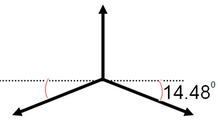
\includegraphics[scale=.6]{/Users/jgates/desktop/latex/pics/explosion1}
\end{floatingfigure}
 
{\bf \Large{\arabic{ProbNum}}} Three ice skaters of equal mass (56 kg) stand together motionless in the center of the rink.  They put their hands together and push off of each other, traveling in three different directions, as shown. The skater on the top of the diagram is traveling ${3.2~\tfrac{m}{s}}$ after they push.

\bigskip
How fast are the other skaters traveling after the push?\paragraph{}
\noindent
\vfill

If the push lasted for 220 ms, determine the average force exerted on the skater at the top of the diagram by the others.

\vfill
%\hfill 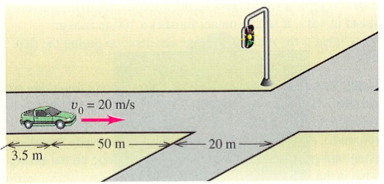
\includegraphics[scale=.85]{/Users/jgates/desktop/latex/pics/redlight.png}
\newpage
